
% \begin{table}[ht]
%     \centering
%     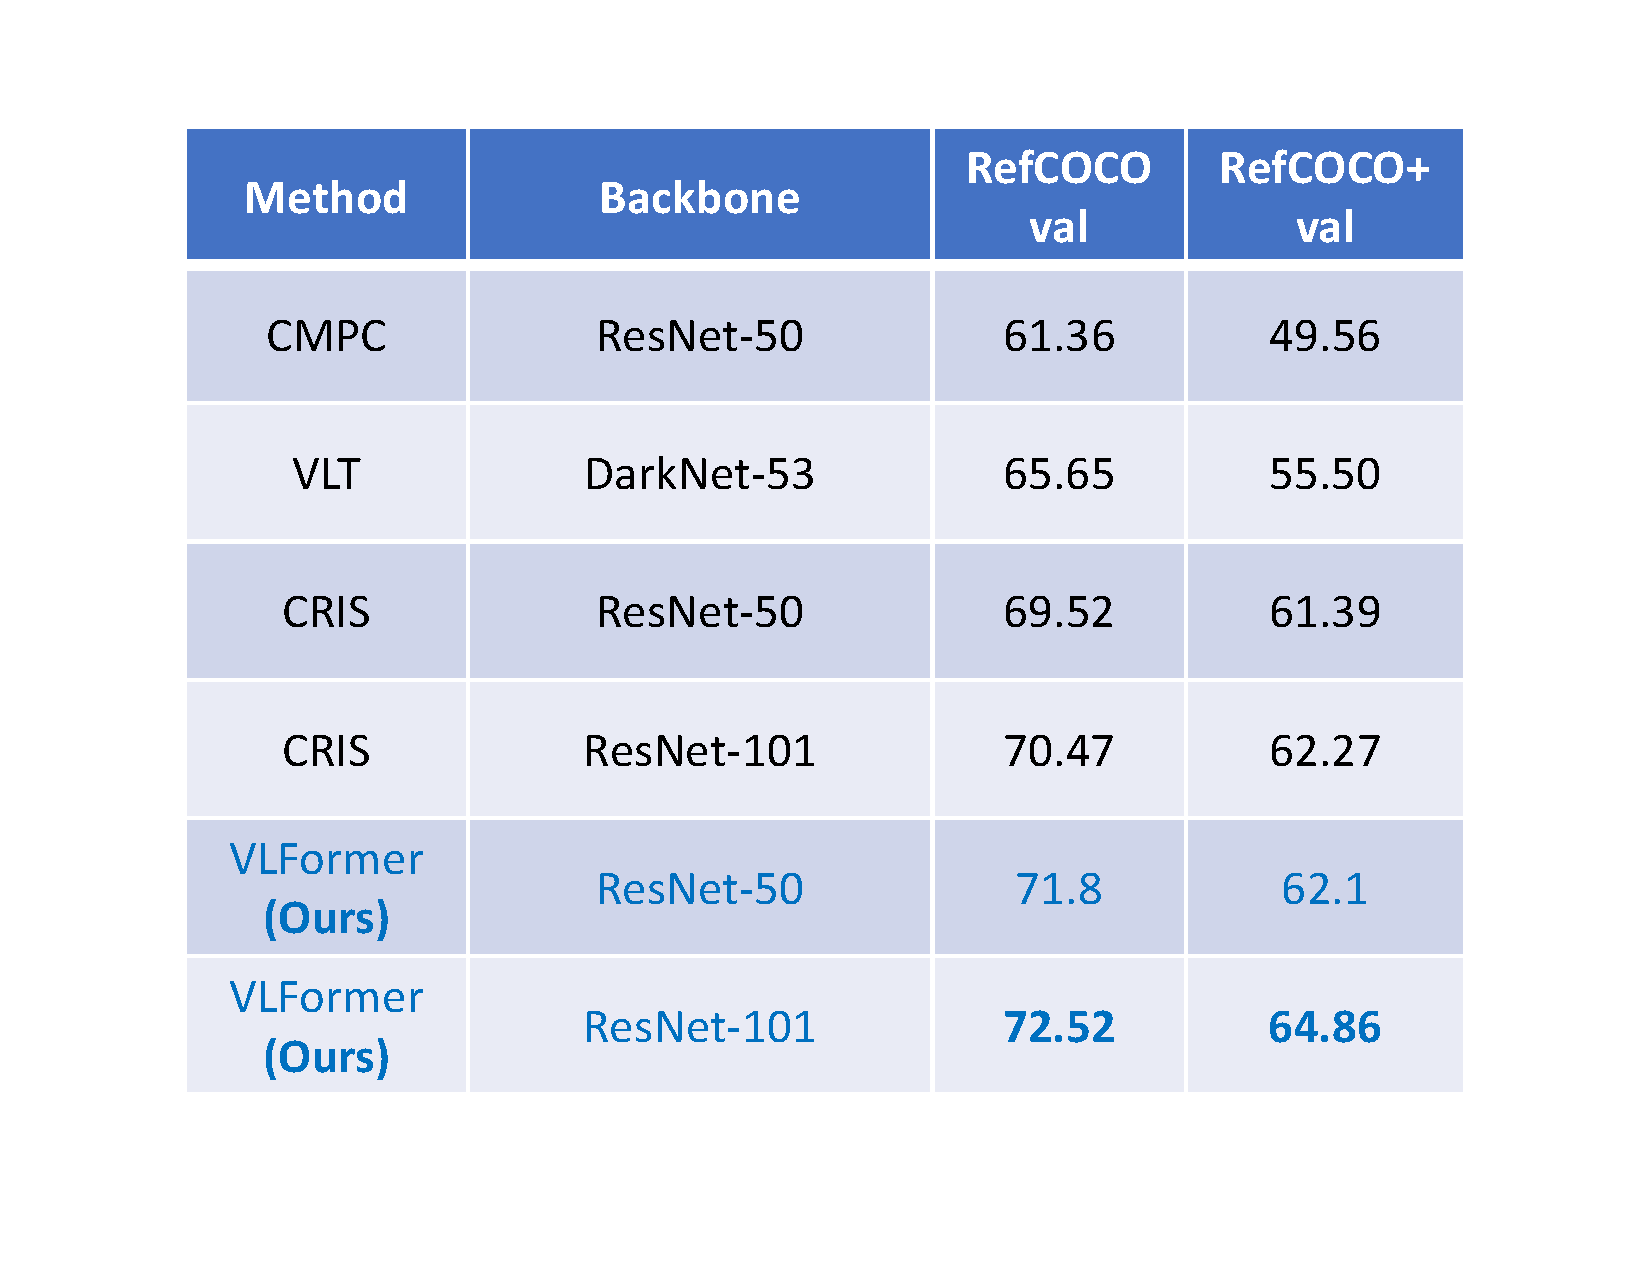
\includegraphics[width=\textwidth]{content/resources/images/referring_segmentation/RefCOCO-SOTA.pdf}
%     \caption{Comparison with the state-of-the-art methods on RefCOCO dataset.}
%     \label{tab:refcoco}
% \end{table}

 
\begin{table*}[ht]
\centering
\begin{tabular}{c|c|ccc|ccc}
\toprule

\multirow{2}{*}{Method} & \multirow{2}{*}{Backbone} & \multicolumn{3}{c|}{RefCOCO} & \multicolumn{3}{c}{RefCOCO+} \\ \cline{3-8} 
                        &                           & val      & testA   & testB   & val      & testA    & testB      \\ \midrule
MAttNet~\cite{yu_mattnet_2018}                    & ResNet-101                & 56.51    & 62.37   & 51.70   & 46.67    & 52.39    & 40.08          \\
NMTree~\cite{liu_learning_2019}                    & ResNet-101                & 56.59    & 63.02   & 52.06   & 47.40    & 53.01    & 41.56          \\
CMSA~\cite{ye_cross-modal_2019}                    & ResNet-101                & 58.32    & 60.61   & 55.09   & 43.76    & 47.60    & 37.89           \\
Lang2Seg~\cite{chen_referring_2019}                    & ResNet-101                & 58.90    & 61.77   & 53.81   & -    & -    & -            \\
CMPC~\cite{huang_referring_2020} & ResNet-101                & 61.36    & 64.53   & 59.64   & 49.56    & 53.44    & 43.23          \\
EFNet~\cite{feng_encoder_2021}                    & ResNet-101                & 62.76    & 65.69   & 59.67   & 51.50    & 55.24    & 43.01         \\
VLT~\cite{ding_vision-language_2021}                     & DarkNet-53                & 65.65    & 68.29   & 62.73   & 55.5     & 59.2     & 49.36     \\
ReSTR~\cite{kim_restr_2022}                   & ViT-B-16                  & 67.22    & 69.3    & 64.45   & 55.78    & 60.44    & 48.27       \\
CRIS~\cite{wang_cris_2022}                    & ResNet-101                & 70.47    & 73.18   & 66.1    & 62.27    & 68.08    & 53.68    \\
LAVT~\cite{yang_lavt_2022}                    & Swin-B                    & 72.73    & 75.82   & 68.79   & 62.14    & 68.38    & 55.1        \\ \midrule
VLFormer\textbf{(Ours)}                    & ResNet-50                    & 73.92    & 76.03   & \textbf{70.86}   & 64.02    & 69.74    & 55.04        \\ 
VLFormer\textbf{(Ours)}                     & ResNet-101                & \textbf{74.67}    & \textbf{76.8}    & 70.42   & \textbf{64.80}    & \textbf{70.33}    & \textbf{56.33}       \\
\bottomrule
\end{tabular}


\caption{Comparisons with the state-of-the-art approaches on RefCOCO and RefCOCO+ benchmarks. We report the results of our method with various visual backbones. IoU is used as the main metric, and  ``-'' shows that the result is not available. The best performance is marked in boldface.}
\label{tab:sota}
\end{table*}


\begin{table*}[ht]
\centering
\begin{tabular}{c|c|cc}
\toprule

\multirow{2}{*}{Method} & \multirow{2}{*}{Backbone} & \multicolumn{2}{c}{G-Ref} \\ \cline{3-4} 
                        &                           & val         & test        \\ \midrule
MAttNet~\cite{yu_mattnet_2018}                    & ResNet-101                   & 47.64           & 48.61          \\
NMTree~\cite{liu_learning_2019}                    & ResNet-101                & 46.59           & 47.88           \\
Lang2Seg~\cite{chen_referring_2019}                    & ResNet-101                  & 46.37           & 46.95           \\

VLT~\cite{ding_vision-language_2021}                     & DarkNet-53                 & 52.99       & 56.65       \\
ReSTR~\cite{kim_restr_2022}                   & ViT-B-16                    & 54.48       & -           \\
CRIS~\cite{wang_cris_2022}                    & ResNet-101                 & 59.87       & 60.36       \\
LAVT~\cite{yang_lavt_2022}                    & Swin-B                     & 61.24       & 62.09       \\ \midrule
VLFormer\textbf{(Ours)}                    & ResNet-50                    & 65.69       & 65.90       \\ 
VLFormer\textbf{(Ours)}                     & ResNet-101 & \textbf{66.77}       & \textbf{66.52}       \\
\bottomrule
\end{tabular}


\caption{Comparisons with the state-of-the-art approaches on G-Ref dataset. We report the results of our method with various visual backbones. IoU is used as the main metric, and  ``-'' shows that the result is not available. The best performance is marked in boldface.}
\label{tab:sota2}
\end{table*}